\documentclass[tikz,border=10pt]{standalone}

\usepackage[utf8]{inputenc}
\usepackage{tikz}
\usetikzlibrary{arrows}
\usetikzlibrary{patterns}
\usetikzlibrary{intersections}
\usepackage{amsmath, amssymb, amsthm}


\title{Your Title Here}
\author{Your Name Here}
\date{\today}

\begin{document}

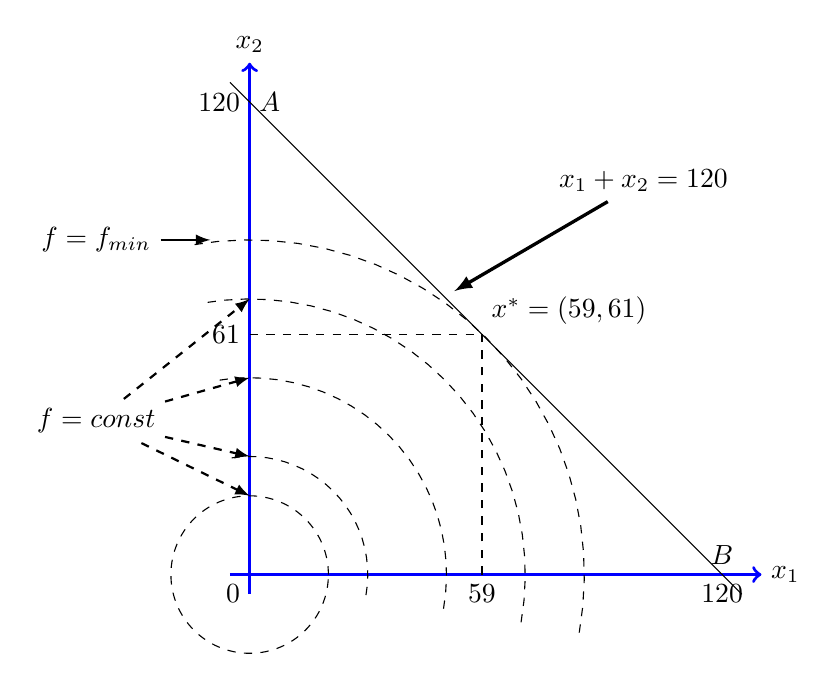
\begin{tikzpicture}
    \draw [blue, ->, very thick, scale = 0.05] (-5,0) -- (130,0);
    \node [right] at (13/2,0) {$x_1$};

    \draw [blue, ->, very thick, scale = 0.05] (0,-5) -- (0,130);
    \node [above] at (0,13/2) {$x_2$};

    \node [below left] at (0,0) {$0$};

    \draw [scale = 0.05] (-5,125) -- (125,-5);
    \node [below] at (12/2, 0) {$120$};
    \node [left] at (0, 12/2) {$120$};

    \node [right] at (0, 12/2) {$A$};
    \node [above] at (12/2, 0) {$B$};

    \node (cor) at (5, 5) {$x_1 + x_2 = 120$};
    \draw [-latex, very thick] (cor) -- (52*0.05, 72*0.05);

    % x∗ = (59, 61)
    \node [above right] at (59*0.05, 61*0.05) {$x^* = (59, 61)$};
    \draw [dashed, scale = 0.05] (59,0) -- (59, 61);
    \draw [dashed, scale = 0.05] (0,61) -- (59, 61);
    \node [below] at (59*0.05, 0) {$59$};
    \node [left] at (0, 61*0.05) {$61$};

    % how can i draw a portion of a circle?
    % You can use the parametrization
    %  x(t)=a+r*cos(t)
    %  y(t)=b+r*sin(t)

    \draw [dashed, domain=-10:100] plot ({1.5*cos(\x)}, {1.5*sin(\x)});
    \draw [dashed, domain=-10:100] plot ({2.5*cos(\x)}, {2.5*sin(\x)});
    \draw [dashed, domain=-10:100] plot ({3.5*cos(\x)}, {3.5*sin(\x)});
    \draw [dashed, domain=-10:100] plot ({85*0.05*cos(\x)}, {85*0.05*sin(\x)});

    % f = const on 4 smaller portions
    \node (constf) at (-39*0.05, 39*0.05) {$f = const$};
    \draw [-latex, thick, dashed] (constf) -- (0, 1);
    \draw [-latex, thick, dashed] (constf) -- (0, 1.5);
    \draw [-latex, thick, dashed] (constf) -- (0, 2.5);
    \draw [-latex, thick, dashed] (constf) -- (0, 3.5);

    % f = f_min on the largest portion
    \node (fmin) at (-39*0.05, 85*0.05) {$f = f_{min}$};
    \draw [-latex, thick,] (fmin) -- (-10*0.05, 85*0.05);

    \draw [dashed] (0,0) circle(1);
\end{tikzpicture}

\newpage
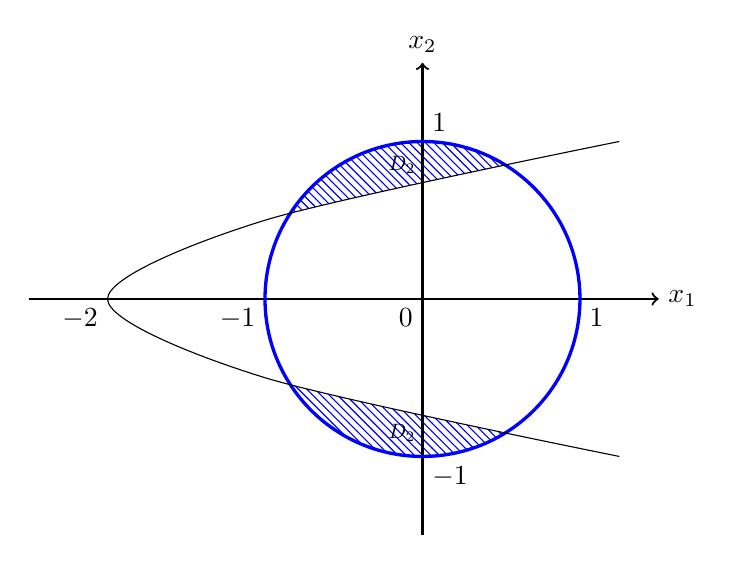
\begin{tikzpicture} [scale = 2]

    \begin{scope}
        \clip (0,0) circle (1);
        \begin{scope} [even odd rule]
            \fill[pattern=north west lines, pattern color=blue] (0,0) circle (1) plot[smooth] coordinates {
            (1.25, 1) (-1, 0.5) (-2, 0) (-1, -0.5) (1.25, -1) };
        \end{scope}
    \end{scope}

    \draw [->, thick] (-2.5,0) -- (1.5,0);
    \draw [->, thick] (0,-1.5) -- (0,1.5);
    \node [right] at (1.5,0) {$x_1$};
    \node [above] at (0,1.5) {$x_2$};
    \node [below left] at (0,0) {$0$};
    \node [below right] at (1,0) {$1$};
    \node [above right] at (0,1) {$1$};
    \node [below left] at (-1,0) {$-1$};
    \node [below right] at (0,-1) {$-1$};
    \node [below left] at (-2,0) {$-2$};

    \draw [blue, very thick] (0,0) circle(1);

    \draw plot[smooth, very thick] coordinates {
    (1.25, 1) (-1, 0.5) (-2, 0) (-1, -0.5) (1.25, -1) };

    %node the intersection between the plot and the x_2 axis
    \node [above left, scale = 0.75] at (0, 0.75) {$D_2$};
    \node [below left, scale = 0.75] at (0, -0.75) {$D_2$};

\end{tikzpicture}

\newpage
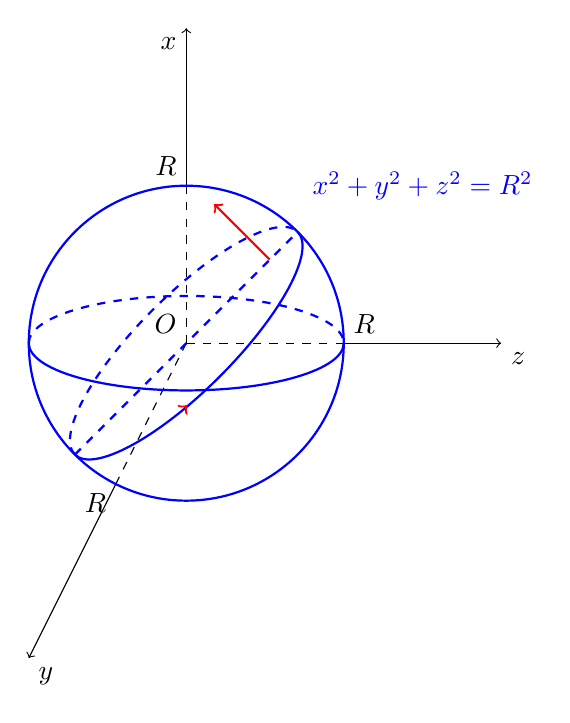
\begin{tikzpicture}
    % we're going 3d today
    \draw [->, name path = z] (2,0) -- (4,0);
    \draw [dashed] (0,0) -- (2,0);
    \draw [->, name path = x] (0,2) -- (0,4);
    \draw [dashed] (0,0) -- (0,2);
    \draw [->, name path = y] (-0.85, -1.7) -- (-2, -4);
    \draw [dashed] (0,0) -- (-0.85, -1.7);

    \node [above left] at (0, 0) {$O$};
    \node [below left] at (0, 4) {$x$};
    \node [below right] at (-2, -4) {$y$};
    \node [below right] at (4, 0) {$z$};
    
    \draw [blue, thick, name path = cir] (0,0) circle (2);
    % arc so it looks 3d
    \draw [blue, thick] (-2,0) arc (180:360:2 and 0.6);
    \draw [blue, thick, dashed] (-2,0) arc (180:0:2 and 0.6);
    % same thing but rotate 45 degrees
    \draw [blue, thick, rotate = 45] (-2, 0) arc (180:360:2 and 0.6);
    \draw [blue, thick, dashed, rotate = 45] (-2, 0) arc (180:0:2 and 0.6);
    \draw [blue, thick, dashed, rotate = 45] (-2, 0) -- (2, 0);
    \draw [red, ->, thick, rotate = 45] (1.5, 0) -- (1.5, 1);
    \draw [red, ->, thick] (0, -0.8) -- (0.01, -0.79); %bad hack
    \node [blue] at (3, 2) {$x^2 + y^2 + z^2 = R^2$};

    \fill[name intersections = {of = x and cir}] 
        (intersection-1) node[above left] {$R$};
    \fill[name intersections = {of = y and cir}]
        (intersection-1) node[below left] {$R$};
    \fill[name intersections = {of = z and cir}]
        (intersection-1) node[above right] {$R$};
\end{tikzpicture}

\newpage

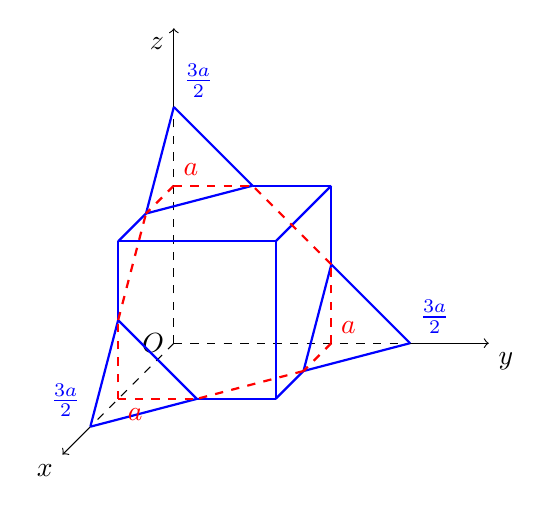
\begin{tikzpicture}
    % another 3d plot
    % thank god it's not a sphere this time
    \draw [->] (3,0) -- (4,0);
    \draw [dashed] (0,0) -- (3,0);
    \draw [->] (0,3) -- (0,4);
    \draw [dashed] (0,0) -- (0,3);
    % give me a moment, i'm reading textbooks from 11th grade
    % why am i doing this to myself, i can literally boot up AutoCAD and do this in 5 minutes
    % Hình chiếu trục đo xiên góc cân
    \draw [->] ({-1.5/sqrt(2)}, {-1.5/sqrt(2)}) -- ({-2/sqrt(2)}, {-2/sqrt(2)});
    \draw [dashed] (0,0) -- ({-1.5/sqrt(2)}, {-1.5/sqrt(2)});
    
    \node [left] at (0, 0) {$O$};
    \node [below left] at (0, 4) {$z$};
    \node [below left] at ({-2/sqrt(2)}, {-2/sqrt(2)}) {$x$};
    \node [below right] at (4, 0) {$y$};

    \coordinate (X_1) at ({-1/sqrt(2)}, {-1/sqrt(2)});
    \coordinate (X_2) at ({-1.5/sqrt(2)}, {-1.5/sqrt(2)});
    \coordinate (Y_1) at (2, 0);
    \coordinate (Y_2) at (3, 0);
    \coordinate (Z_1) at (0, 2);
    \coordinate (Z_2) at (0, 3);

    \coordinate (XY_1) at ({2-0.5/sqrt(2)}, {-0.5/sqrt(2)});
    \coordinate (XY_2) at ({1-1/sqrt(2)}, {-1/sqrt(2)});
    \coordinate (XY_3) at ({2-1/sqrt(2)}, {-1/sqrt(2)});
    \coordinate (YZ_1) at (2, 1);
    \coordinate (YZ_2) at (1, 2);
    \coordinate (YZ_3) at (2, 2);
    \coordinate (XZ_1) at ({-1/sqrt(2)}, {-1/sqrt(2)+1});
    \coordinate (XZ_2) at ({-0.5/sqrt(2)}, {-0.5/sqrt(2)+2});
    \coordinate (XZ_3) at ({-1/sqrt(2)}, {-1/sqrt(2)+2});
    \coordinate (XYZ) at ({2-1/sqrt(2)}, {2-1/sqrt(2)});

    \draw [blue, thick] (X_2) -- (XZ_1);
    \draw [blue, thick] (X_2) -- (XY_2);
    \draw [blue, thick] (Y_2) -- (YZ_1);
    \draw [blue, thick] (Y_2) -- (XY_1);
    \draw [blue, thick] (Z_2) -- (YZ_2);
    \draw [blue, thick] (Z_2) -- (XZ_2);

    \draw [blue, thick] (XY_1) -- (YZ_1);
    \draw [blue, thick] (XZ_1) -- (XY_2);
    \draw [blue, thick] (YZ_2) -- (XZ_2);

    \draw [blue, thick] (YZ_2) -- (YZ_3);
    \draw [blue, thick] (XY_2) -- (XY_3);
    \draw [blue, thick] (XZ_2) -- (XZ_3);

    \draw [blue, thick] (XYZ) -- (YZ_3);
    \draw [blue, thick] (XYZ) -- (XY_3);
    \draw [blue, thick] (XYZ) -- (XZ_3);

    \draw [blue, thick] (XY_1) -- (XY_3);
    \draw [blue, thick] (XZ_1) -- (XZ_3);
    \draw [blue, thick] (YZ_1) -- (YZ_3);

    \draw [red, dashed, thick] (X_1) -- (XY_2);
    \draw [red, dashed, thick] (X_1) -- (XZ_1);
    \draw [red, dashed, thick] (Y_1) -- (YZ_1);
    \draw [red, dashed, thick] (Y_1) -- (XY_1);
    \draw [red, dashed, thick] (Z_1) -- (YZ_2);
    \draw [red, dashed, thick] (Z_1) -- (XZ_2);

    \draw [red, dashed, thick] (XY_1) -- (XY_2);
    \draw [red, dashed, thick] (XZ_1) -- (XZ_2);
    \draw [red, dashed, thick] (YZ_1) -- (YZ_2);

    \node [red, below right] at (X_1) {$a$};
    \node [red, above right] at (Y_1) {$a$};
    \node [red, above right] at (Z_1) {$a$};

    \node [blue, above left] at (X_2) {$\frac{3a}{2}$};
    \node [blue, above right] at (Y_2) {$\frac{3a}{2}$};
    \node [blue, above right] at (Z_2) {$\frac{3a}{2}$};

    % took me 3 hours to figure out how to draw this
    % i'm not even joking
    % in retrospect, i shouldn't have joined this course
    % maybe i would be richer, happier
    % this is so frustrating
    % https://www.youtube.com/live/ukJ1ZQxtPaY?si=S0_pqRnXXsXXLs3K&t=5189

\end{tikzpicture}
\end{document}